\begin{frame}{What is Python?\footnote{https://en.wikipedia.org/wiki/Python\_(programming\_language)} }
  Python is an interpreted high-level general-purpose programming language. Its design philosophy emphasizes code readability with its use of significant indentation. Its language constructs as well as its object-oriented approach aim to help programmers write clear, logical code for small and large-scale projects.
\pause
\vspace{0.6cm}
\begin{figure}

\includegraphics[width=3.5cm,height=3.5cm,keepaspectratio]{img/python_logo.png}
\end{figure}


\end{frame}
\begin{frame}
  \tit{Who created Python?}
  Python was created by Guido van Rossum in the Netherlands in 1990. Van Rossum developed  Python as a hobby, and Python has become a popular programming language widely used in industry and academia due to its simple, concise, and intuitive syntax and extensive library.
  

\end{frame}
\begin{frame}
  \tit{Why Python?}
  Because of many reasons\footnote{https://www.quora.com/Why-do-people-still-use-Python}:
\begin{itemize}
  \item  \textbf{Easy to learn:} Learning Python is nothing but learning English.\pause
  \item  \textbf{ Used everywhere:} Python is used in AI, ML(Artificial Intelligence and Machine Learning). It is also used in data science, games, apps, websites, automation, etc.\pause
  \item  \textbf{ General purpose programming language:} It is a general purpose programming language which means it can be used on all devices and also in many different situations.\pause
  \item  \textbf{ Loads of libraries:} Want to solve algebraic equations? Use numpy. Want to deal with images? Use PIL.\pause
  \item \textbf{Just few lines of code does great:} With Python in just 5 lines of code is equivalent to, say, 20 lines of PHP code.\pause
  \item  \textbf{ Great community:} Many people are willing to help with issues regarding Python. There is a great community.
    
\end{itemize}

\end{frame}
\begin{frame}
  \tit{Why Python?\footnote{https://becominghuman.ai/why-is-python-so-popular-b01a006b2be4}}

 \begin{center}
    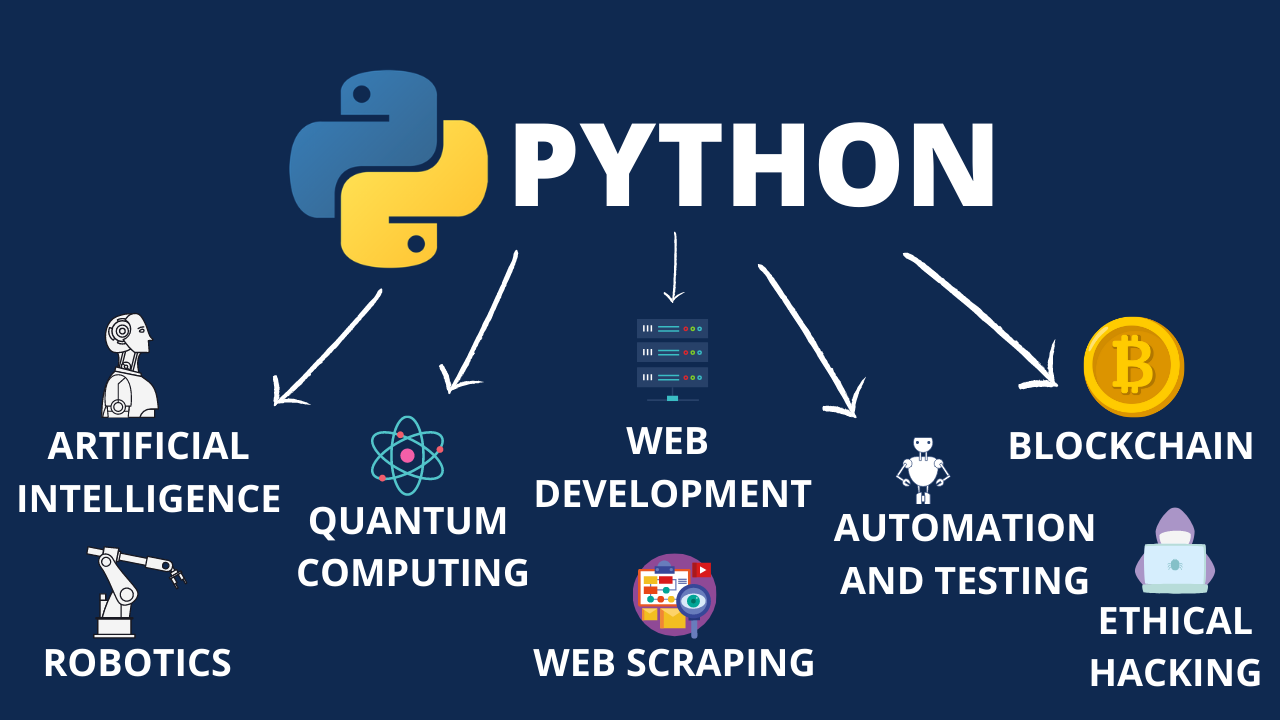
\includegraphics[scale=0.25]{img/why_python.png}
 \end{center}

\end{frame}
\begin{frame}
  \tit{Why Python?}

 \begin{center}
    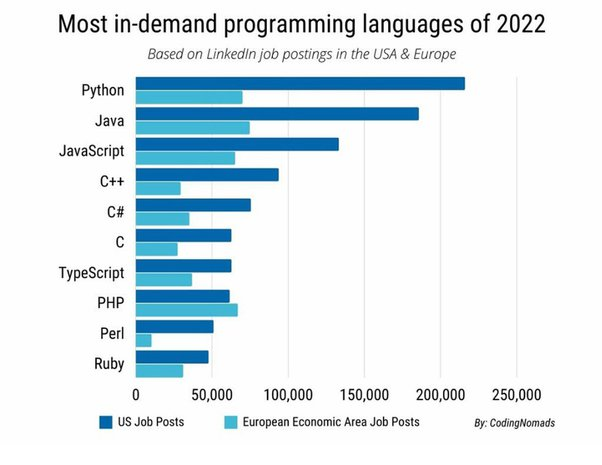
\includegraphics[scale=0.5]{img/most_demand.jpeg}
 \end{center}

\end{frame}
\begin{frame}
  \tit{Why Python?}

 \begin{center}
    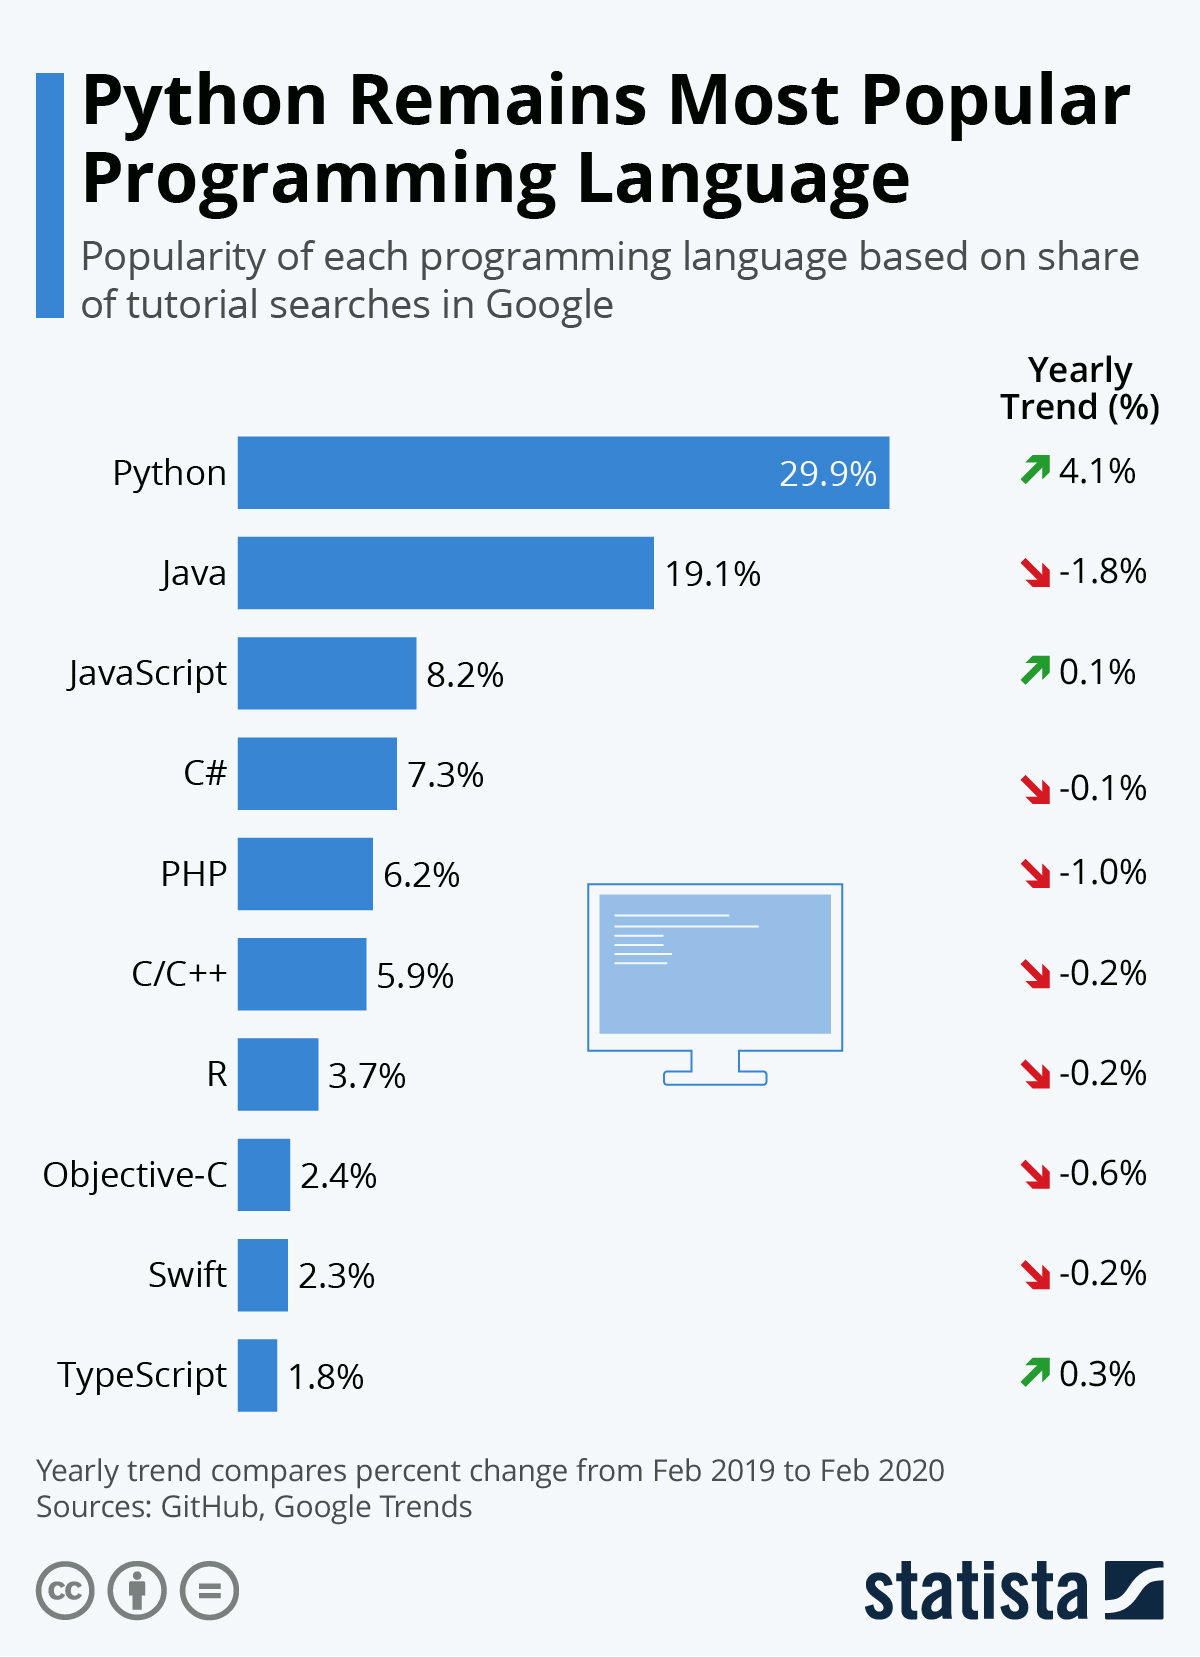
\includegraphics[scale=0.13]{img/most_popular.jpeg}
 \end{center}

\end{frame}
\begin{frame}
  \tit{What is an open source/free software?\footnote{https://en.wikipedia.org/wiki/Free\_and\_open-source\_software}}
  Free and open-source software (FOSS) is software that is both free software and open-source software[a] where anyone is freely licensed to use, copy, study, and change the software in any way, and the source code is openly shared so that people are encouraged to voluntarily improve the design of the software.
  \pause \\
  Examples of free software: \textbf{VLC Media}, \textbf{Linux Mint}, \textbf{Gimp}, \textbf{Firefox}, ... etc.

% \end{frame}
% \begin{frame}{Logiciel Libre \footnote{https://en.wikipedia.org/wiki/Free\_software}}
%   Free software (or libre software) is computer software distributed under terms that allow users to run the software for any purpose as well as to study, change, and distribute it and any adapted versions. 
% \pause
\vspace{1cm}
\begin{figure}

\includegraphics[width=3cm,height=2.5cm,keepaspectratio]{img/gnu.png}
\end{figure}

\end{frame}
\begin{frame}{What is a Licence?}
  A software license is a contract by which the copyright holder of a computer program defines with his co-contractor (operator or user) the conditions under which this program may be used, distributed or modified.
\end{frame}
\begin{frame}{GNU Licence\footnote{https://en.wikipedia.org/wiki/GNU\_General\_Public\_License}}
  The GNU General Public License (GNU GPL or simply GPL) is a series of widely used free software licenses that guarantee end users the four freedoms to run, study, share, and modify the software.

\pause
\vspace{1cm}
\begin{figure}

\includegraphics[width=3cm,height=2.5cm,keepaspectratio]{img/GPLv3.png}
\end{figure}

\end{frame}
\begin{frame}
  \tit{Levels of freedom of a software}
\pause
  \begin{center}
      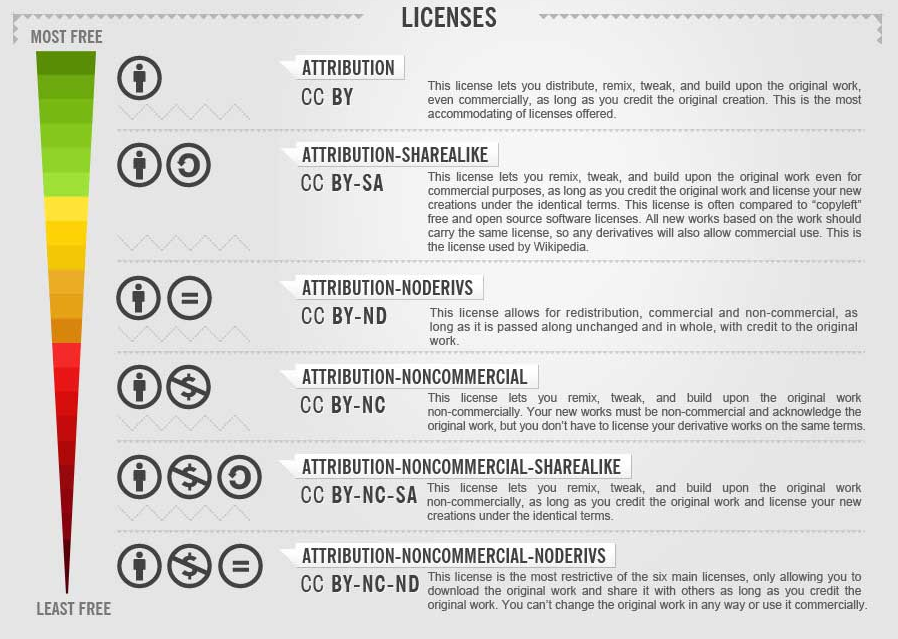
\includegraphics[scale=0.44]{img/creative-commons2.png}
  \end{center}


\end{frame}
\begin{frame}
  \tit{Is there other types of licences?}
\pause
\begin{center}
      \includegraphics[scale=0.3]{img/table_comp.png}
\end{center}
\end{frame}
\begin{frame}
  \tit{What we will study during the semester}

\begin{center}
  \resizebox{.5\linewidth}{!}{
  \smartdiagram[descriptive diagram]{
    {Chap 1,{Introduction to computers, Programs and Python}},
    {Chap 2, {Elementary Programming}}, 
    {Chap 3, {Mathematical Functions and Strings}},
    {Chap 4,{ Conditions}},
    {Chap 5, {Loops}}, }}
\end{center}

\end{frame}
\begin{frame}
  \tit{What we will study during the semester}
\begin{center}
  \resizebox{.5\linewidth}{!}{
  \smartdiagram[descriptive diagram]{
    {Chap 6, Functions},
    {Chap 7, Lists},
    {Chap 8, {Tuples, Sets and Dictionaries}},
    {Chap 9, Multidimensional Lists},
    {Chap 10, Files and Exceptions Handling}}}
\end{center}

\end{frame}
% \begin{frame}
%   \tit{Python 2 Vs Python 3}

  

% \end{frame}
\begin{frame}
  \tit{Differents ways to run Python}

\begin{itemize}
  \item Interactive Mode (Command prompt).\pause
  \item Command Line (File running)  'python file.py'. \pause
  \item Text Editor (VS Code, Jupyter). \pause
  \item IDE (PyCharm)
\end{itemize}
  

\end{frame}
\begin{frame}
  \tit{Type of Errors}

  \begin{itemize}
    \item \textbf{Syntax errors} result from errors in code construction, such as mistyping a statement, incor-
rect indentation, omitting some necessary punctuation, or using an opening parenthesis with-
out a corresponding closing parenthesis.
    \item \textbf{Runtime errors} are errors that cause a program to terminate abnormally. They occur while a
    program is running if the Python interpreter detects an operation that is impossible to carry
    out.
    \item \textbf{Logic errors} occur when a program does not perform the way it was intended to. Errors of this
    kind occur for many different reasons.
  \end{itemize}

\end{frame}
\begin{frame}
  \tit{Objective of the course}
\begin{block}
  
    At the end of this semester, you will be able to solve a problem and write its code in Python.
  
\end{block}
\end{frame}